By using Eclipse~\cite{eclipse}, EMF~\cite{emf} and Xtext~\cite{xtext} we built a domain specific language that is rich enough to express the policies discovered in the analysis. We developed a grammar that is based on our programming experience, and believed to have a consistent forthcoming syntax and conceptual constructs. Finally, we used our Policy Engine DSL editor to write the policies.

Our model is of considerable size, and consists of the following core packages, differentiated in separate Ecore Diagrams (can be viewed in full in \nameref{sec:appendix-a}); 9 sensors classes and 6 actuators classes (see Figure \ref{fig:ecore-sensors-actuators}), 6 expression language classes (see \ref{fig:ecore-expression-language}), 5 building definition classes (see Figure \ref{fig:ecore-building-definition}) and 10 policy definition classes (see Figure \ref{fig:ecore-policy-definition}).

We have included the full DSL implementation based on two of the interviews, one for Br\"{u}el \& Kj\ae r (see  \nameref{app:bogk}) and one for K\o benhavns Tekniske Skole (see \nameref{app:kts}). Please note that they are fully working implementations running in Eclipse..

\begin{figure}[h]
	\centering
    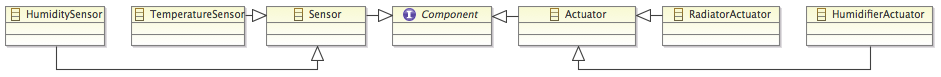
\includegraphics[scale=0.37]{ecore-sensors-actuators.png} 
	\caption{A fragment of the \textit{sensor} and \textit{actuator} metamodel hierarchy. If new types are needed, they should be defined in the metamodel.}
	\label{fig:ecore-sensors-actuators}
\end{figure}

\subsection{Expression language}
After the analysis of the interviews we concluded that the needed expression language needed not to be very advanced. We need boolean variables (\textit{states}), and if-statements with two different types of conditions; the normal if-statement and the one that operates on a timer (see Figure \ref{fig:dsl-conditionalexpression}). 

\begin{figure}[h]
  \centering
    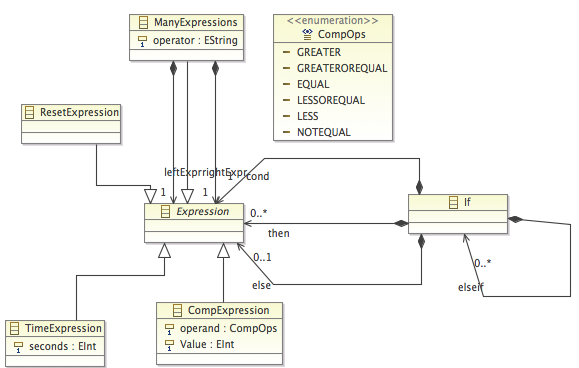
\includegraphics[width=10cm]{ecore-expression-language.png} 
	\caption{The metamodel related to the \textit{expression language}. The inherited class NamedElement has been omitted.}
	\label{fig:ecore-expression-language}
\end{figure}

\pagebreak
\subsection{Building definition}
In order to specify the building(s) with all their floors and rooms, the core classes has been included in Figure ref{fig:ecore-building-definition}. They all inherit from NamedElement, making it possible to give them a name than can be used for later referencing.
\begin{figure}
  \centering 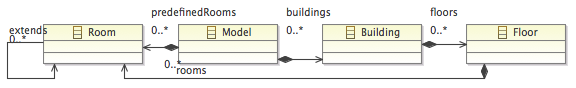
\includegraphics[scale=0.4]{ecore-building-definition.png}  
	\caption{The metamodel related to the \textit{building definition}. The inherited class NamedElement has been omitted.}
	\label{fig:ecore-building-definition}
\end{figure}

\subsection{Policy definition}

\begin{figure}
  \centering
    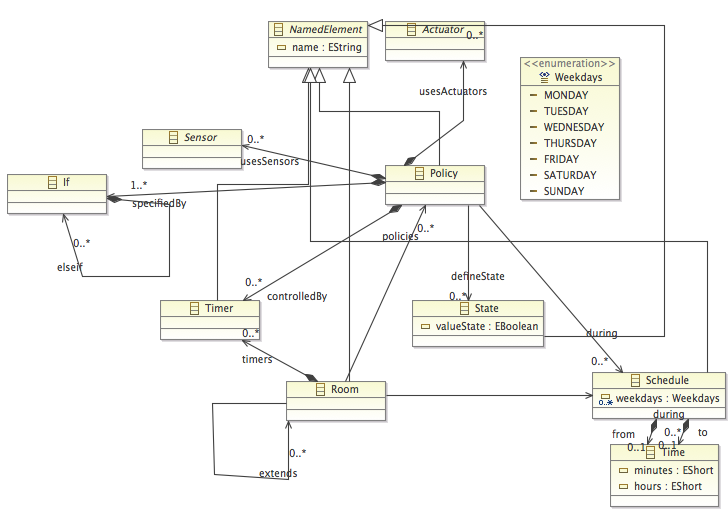
\includegraphics[scale=0.3]{ecore-policy-definition.png}	
	\caption{The metamodel related to the \textit{policy definition}. The inherited class NamedElement has been omitted.}
	\label{fig:ecore-policy-definition}
\end{figure}

\pagebreak
There are several extra classes, consisting of subsystems that can be implemented in future work.

During the analysis of the interviews, different meta-constructs were defined. It was evident that the below three key concepts were needed in order to tailor the policies for the interviewees using the DSL;

\begin{enumerate}
	\item \textit{Time}. Time has to be an integral part of the DSL, and not just related with the internal policy logic. Several interviewees mention concepts like weekdays, weekends, normal working hours, holidays, night, day, morning etc.
	
	\item \textit{Building specification}. It should be possible to define the buildings, their floors, number and types of rooms etc.

	\item \textit{Policy}. The actual behavior, ie. adjusting actuators based on sensor input, needs to be defined. 
\end{enumerate}

\subsection{Time}\label{subsec:time}
The analysis of the interviews clearly shows that Time is necessary. We have extrapolated the need for Time in two different cases;
	\begin{enumerate}
		\item Time conditional expression - an expression used for determining the flow of a behavior.
		\item Schedules - types that define a timespan which can later be attached to a specific behavior.
	\end{enumerate}

\subsubsection{Time conditional expression}\label{subsubsec:conditionalexpression}
A \textit{time conditional expression} is an `if' statement that can react based on a built-in timer function. 

\begin{figure}
  \centering
    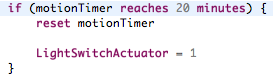
\includegraphics[scale=.5]{dsl-conditional-time-expression.png} 
	\caption{An example of a \textit{time conditional expression} that evaluates to true if more than 20 minutes have passed.}
	\label{fig:dsl-conditionalexpression}
\end{figure}

\newpage
\subsubsection{Schedules}\label{subsubsec:schedules}
\textit{Schedules} are predefined types representing a timespan where action or no-action takes place. Note that by defining several The \textit{schedules}, it is possible both to make schedules than can overlap in time, but also policies that takes over when other policies reach their end. 

\begin{figure}
  \centering
  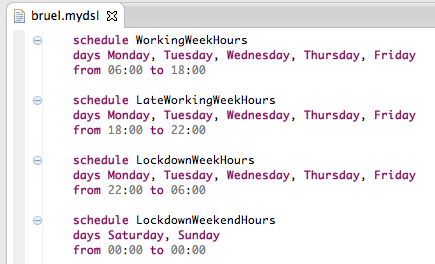
\includegraphics[scale=.5]{dsl-schedules.png}
  \caption{An example of a \textit{schedule} defined for a interviewee.}
  \label{fig:dsl-schedules}
\end{figure}

\subsection{Building specification}\label{subsec:buildingspecification}
Rooms and room types are part of the complete building specification, with terminology rooted in concepts revolving around buildings, ie. rooms, room types, floors, different sensors and actuators. \\

To avoid confusing the DSL user with an overwhelming amount of declarations of rooms, sensors and actuators - we have designed \textit{room types} that declare static use of sensors and actuators. Independent rooms that stick out from the crown can still be defined on an instance level.

\begin{figure}
  \centering
    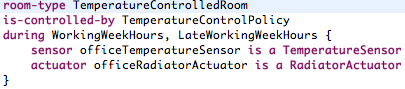
\includegraphics[scale=.5]{dsl-room-types.png}
	\caption{An example of \textit{room types} defined for a interviewee.}
	\label{fig:room-types}
\end{figure}

Building specification as in the example below, helps us map out the actual buildings as they are in our DSL. With this we are able to accurately define exact locations for sensors and actuators as well as implement policies for rooms in specific locations. 

\begin{figure}
  \centering
  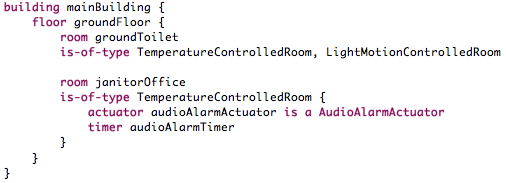
\includegraphics[scale=.5]{dsl-building-definition.png}  
  \caption{An example of \textit{building specification} defined for a interviewee. Note that the janitorOffice inherits from a TemperatureControlled room (which uses a \textit{TemperatureSensor} and a \textit{RadiatorActuator}) but also declares a \textit{AudioAlarmActuator} and a \textit{Timer} instance.}
  \label{fig:dsl-building-definition}
\end{figure}

\subsection{Policy}\label{subsec:policies}
Policies define the actual behavior, ie. adjustment of actuators, based on sensor input. 

\begin{figure}
  \centering
    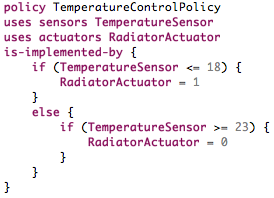
\includegraphics[scale=.5]{dsl-policy-definition.png} 
	\caption{An example of \textit{policy} using a single sensor type and a single actuator type.}
	\label{fig:dsl-policy-definition}
\end{figure}

\section{Evaluation}\label{sec:evaluation}

\subsubsection{Br\"{u}el \& Kj\ae r}\label{subsec:bruel}
The requirements received from Br\"{u}el \& Kj\ae r were implemented in our DSL and can be found in \nameref{sec:dsl-bruel}. One of the requirements from the interview (\textit{all sensor and actuator data stored in a repository for use in a visual display of data in the FM office}) was not implemented in our DSL because we decided to narrow the scope of the project. After evaluating these requirements, we realized that some of the sensors and actuators needed to satisfy the implementation are not defined in our metamodel. While these problems could be easily fixed by simply adding some new classes in the metamodel, we evaluated this area as one that our DSL can be further improved as discussed in \nameref{subsec:def-sensor-actuator-types}.

\subsubsection{K\o benhavns Tekniske Skole}\label{subsec:kts}
The implementation of these requirements in our DSL can be found in \nameref{sec:dsl-kts} and just like in the evaluation in \nameref{subsec:bruel}, we faced the same lack of sensors and actuators. This seems to be a recurring issue in our language but nonetheless it provides a nice opportunity to improve our language. It is further discussed in \nameref{subsec:def-sensor-actuator-types}. 
Another aspect of our language that can be refined is the ability to define how each policy should be used as discussed in \nameref{subsec:during}. 
